\section{Basic plasma physics}\label{sec:grundlagen}

\subsection{Physical properties of plasma}\label{subsec:physicalproperties}

There are several properties which are important for the characterization of plasma. At first of all, one major constraint is that the plasma has to be quasi neutral, i.e. the amount of positive (ions $i$) and negative (electrons $e$) charged particles is approximately equal,
\begin{align}
	\label{eq:quasineutral}
	n_e = \chi_j n_{i,j} \mc
\end{align}
where $n_e$ and $n_{i,j}$ denote the density of electrons and ions, respectively, and $\chi_j$ is the degree of ionization. Potentially, there might be deviation from this condition, but they can only appear on scales small compared to the Debye-length.

\subsection{Debye length}\label{subsec:debyelength}

The Debye length is a characteristic length scale in plasma physics regarding variations in the electrical potential of charged particles which can be derived by means of the Debye"=Hückel"=Theory. If we consider a single negative charge, there will be statistically more positive charged particles shielding the negative one. Hence there will be a decrease in the electrical potential. The Debye length is the length, where the potential dropped on the value $1/e$. It is
\begin{align}
	\label{eq:debyelength}
	\subsc{\lambda}{D} = \sqrt{\frac{\varepsilon_0 \subsc{k}{B}/e^2}{n_e/T_e + \chi_j n_{i,j}/T_j}} \mc
\end{align}
where $T_\alpha$ are the corresponding Temperatures of charged particles. A much more easier form of \eqref{eq:debyelength} is obtained if the ionic temperature is neglected, due to the marginal mobility of the ions. In this approximation,
\begin{align}
	\label{eq:debyelengthsimple}
	\subsc{\lambda}{D} = \sqrt{\frac{\varepsilon_0 \subsc{k}{B} T_e}{n_e e^2}}
\end{align}
is valid. Since the Debye length is only property of electrostatic deviations, another quantity, the plasma frequency can be introduced.

\subsection{Plasma frequency}\label{subsec:plasmafreq}

A local compression is not a state of equilibrium, so the Coulomb interaction is acting on the electrons in such a way, that the equilibrium could be established. Due to the inertia of the electrons, they do not rest in their idle state but overshoot the mark which leads to another compression. This process of collective oscillation happens with the plasma frequency
\begin{align}
	\label{eq:plasmafreq}
	\subsc{\omega}{p} = \sqrt{\frac{n_e e^2}{m_e \varepsilon_0}} \md
\end{align}
Below $\subsc{\omega}{p}$ incident electromagnetic waves are reflected, above $\subsc{\omega}{p}$ incident waves are transmitted through the plasma.

\subsection{Glow discharge}\label{subsec:glowdischarge}

The easiest way to create plasma in laboratories is the apply a voltage between to electrodes in a tube which is filled with a certain gas. Through random processes (for example ionization through cosmic radiation), there is finite number of free electrons and ions in each gas even at room temperature. These free charged particles are accelerated towards the electrodes. If the voltage is sufficiently high and the electrons ionize the atoms or the ions free another electron at the impact on the cathode, a gas charge will occur. This voltage is called the \emph{breakdown voltage}. The breakdown voltage $\subsc{U}{br}$ depends on the gas pressure $p$ and the distance $d$ of the electrodes. These quantities are connected by the \emph{Paschen law} and
\begin{align}
	\label{eq:paschen}
	\subsc{U}{br} = \frac{\alpha p d}{\ln \left( \beta p d \right) + \ln \left[\ln \left( 1+\gamma^{-1} \right)\right]}
\end{align}
holds with gas specific constants $\alpha$ and $\beta$. Figure \ref{fig:paschen} shows possible Paschen curves.
\begin{figure}
	\centering
	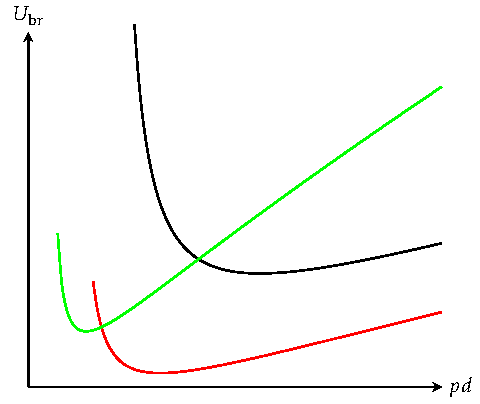
\includegraphics[width=0.5\textwidth]{paschenkurve}
	\caption{\label{fig:paschen}Possible Paschen curves.}
\end{figure}

\subsection{Langmuir probe}\label{subsec:singlelangmuir}

To measure plasma characteristics, the Langmuir probe is the most common device that is used. The probe consists of an electrode inserted into the plasma. Measured are the voltage between the electrode and a reference potential and the current flowing onto or off the probe. The experimental setup is displayed in figure \ref{fig:setup} in configuration \textcircled{{\scriptsize 1}}.
\begin{figure}[tb]
	\centering
	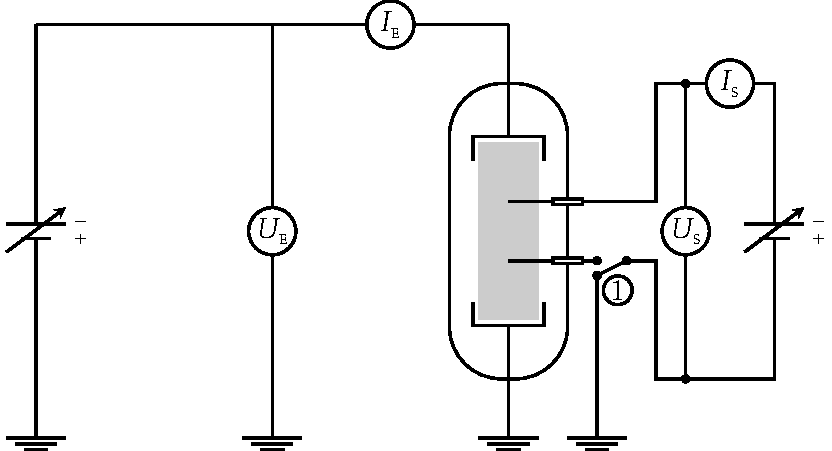
\includegraphics[width=0.5\textwidth]{setup.pdf}
	\caption{\label{fig:setup}Experimental setup with the single and the double probe.}
\end{figure}
Assuming that initially the potential of the probe and the plasma are equal, there will be higher electron flux onto the probe compared to the ion flux due to the different mobilities. After a certain time when the potential is too negative to attract further electrons more ions move onto the probe. The state of equilibrium is when both fluxes are equal and the probe is on the so called \emph{floating potential} $\subsc{U}{fl}$. 

By changing the applied voltage $\subsc{U}{s}$ between a reference potential (for example the cathode) and the probe the characteristic curve can be measured. For high negative voltages, only ions are attracted and the current is limited to the ion saturation current
\begin{align}
	\label{eq:ionsatcurrent}
	\subsc{I}{i, sat} = 0.61 e n_e S \sqrt{\frac{T_e}{m_i}}
\end{align}. 
where $S$ is the probe surface and $m_i$ the ion mass. If the voltage is increased, the probe reaches the floating point, where the current vanishes. A further increase will result in the electron retardation region where more and more electrons are drawn on the tip of the probe. The dependence is exponential and it is
\begin{align}
	\label{eq:electronretardation}
	I = \subsc{I}{e, sat} e^{-e(\subsc{U}{fl} - U)/T_e} + \subsc{I}{i, sat}
\end{align}
with\begin{align}
	\label{eq:electronsatcurrent}
	\subsc{I}{e, sat} = - e n_e S \sqrt{\frac{T_e}{2 \pi m_e}} \md
\end{align}
If the voltage is as large as the plasma potential all electrons in the surrounding are drawn and the current is limited to the electron saturation current $\subsc{I}{e, sat}$. Yet, there is a dependence on the surface of the probe tip that, in general, there will be no saturation due to the increasing boundary layer between probe and plasma and the higher electron flux coming along. A characteristic curve is plotted in figure \ref{fig:langmuirsingle}.
\begin{figure}[tb]
	\centering
	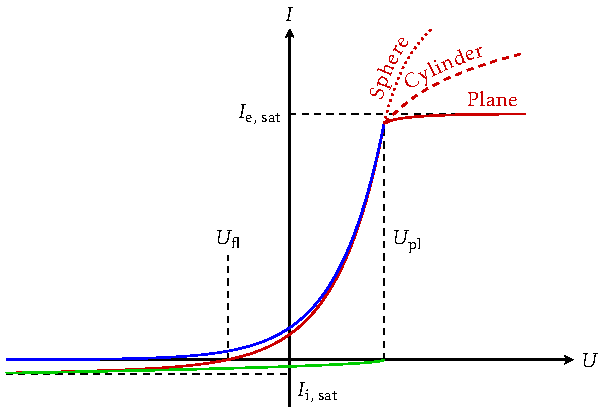
\includegraphics[width=0.5\textwidth]{langmuirsonde.pdf}
	\caption{\label{fig:langmuirsingle}Typical characteristic curve of a single Langmuir probe. The green line is the ion current, the blue one is the electron current and the red one is the combined current.}
\end{figure}
The electron temperature and density for the calculation of the degree of ionization, Debye length and plasma frequency are obtained by fitting the the exponential dependence \eqref{eq:electronretardation} in the electron retardation regime to experimental data.

\subsection{Double probe}\label{subsec:doubleprobe}

Sometimes the single probe fails, for example when there is no well defined reference potential, the double probe is used. The mechanism is the same as for the single probe but the characteristic curve looks a little bit different. We define $U=U_1 - U_2$, so a negative voltage means that the second probe has a more negative potential to the plasma potential than probe 1, so its ion current will be increased. If it is sufficiently negative, only ions are attracted and the electron current is given by $\subsc{I}{i, sat}^2$. When the point $I=0$ (both probes are on the floating potential) is approached, the range of electron retardation is reached and the current depends linear on the applied voltage. If the probes are equal in size and shape, the characteristic curve is symmetric around $I=U=0$. Figure \ref{fig:doubleprobe} depicts a characteristic curve of a double probe.
\begin{figure}[tb]
	\centering
	\includegraphics[width=0.5\textwidth]{doppelsonde.pdf}
	\caption{\label{fig:doubleprobe}Typical characteristic curve of a single Langmuir probe. The green line is the ion current, the blue one is the electron current and the red one is the combined current.}
\end{figure}
For the double probe, the electron temperature is obtained by extrapolation for the saturation currents $\subsc{I}{i, sat}^{1,2}$ as depicted in figure \ref{fig:doubleprobe}. Further, the slope at $U=0$ has to be determined by a linear fit. These three parameters are the input for the conditional equation for the electron temperature, namely
\begin{align}
	\label{eq:doubleprobeelectrontemp}
	T_e = \left( \left. \frac{\d I}{\d U} \right|_{U=0} \right)^{-1} e \frac{\subsc{I}{i, sat}^1 \subsc{I}{i, sat}^2}{\subsc{I}{i, sat}^1 + \subsc{I}{i, sat}^2} \md
\end{align}
By using equation \eqref{eq:ionsatcurrent} the density can be calculated.
